%\documentclass[twoside, a4paper, DIV=11, bibliography=totocnumbered]{scrreprt}
\documentclass[twoside, a4paper, DIV=11, open=any, bibliography=totoc]{scrbook}

\usepackage{url}
\usepackage{hyperref}
\usepackage{graphicx}
\usepackage[all]{hypcap}
\usepackage[utf8]{inputenc}
\usepackage[ngerman]{babel}
\usepackage[skipabove=\baselineskip,skipbelow=\baselineskip,outermargin=30pt,innermargin=30pt]{mdframed}

\usepackage{mdframed}

\usepackage{blindtext} % remove this one, only for template/demonstration

\hypersetup
{
 pdfauthor={Vorname Name},
 pdftitle={Seminararbeit ... },
 pdfkeywords={...},
 colorlinks=true,
 citecolor=black,
 filecolor=black,
 linkcolor=black,
 urlcolor=black
}

\KOMAoption{headings}{normal}

\tolerance=4000
\emergencystretch=20pt

\begin{document}

%*************************************************************************
\begin{titlepage}
    \subject{LVA: "`Technik für Menschen 2040"'}
    \title{Literaturarbeit, Übungskritik \& Szenario 2040}
    \author{
        Florian Schager\\
        \small 11819578
    }
    \date{\today}
    \titlehead{Sommersemester 2021}
\end{titlepage}
\maketitle
%*************************************************************************



\tableofcontents


%*************************************************************************
%*************************************************************************
\chapter{Über den Autor} \label{chap:Autor}

\section{Stammdaten} \label{sec:stammdaten}

Name: Florian Schager\\
MatNr: 11819578\\
Studium: Bachelorstudium Technische Mathematik \\
Semester: 6.Semester \\

\section{Freiwillige Selbstbeschreibung} \label{sec:selbstbeschreibung}

\textit{Freiwillig: ein paar Worte der Selbstbeschreibung}

\begin{itemize}
    \item Was interessiert mich an meinem Studium, warum habe ich es gewählt?
    \item Welche Themen und Gedanken beschäftigen mich?
    \item Warum habe ich diese LVA gewählt?
    \item Interesse auch in Zukunft vernetzt zu bleiben, um wichtige Zukunftsthemen zu diskutieren?
    \item Interesse an Bakk-/Diplomarbeit, Praktikum etc.?
    \item Kontaktinformation, Email, Webseite, Twitter
\end{itemize}


etc.

%*************************************************************************
%*************************************************************************
\chapter{Literaturarbeit} \label{chp:LitKrit}

\section{Literatur-Gruppe} \label{sec:litgruppe}

Die Literaturarbeit wurde in Gruppe ... durchgeführt. Mitglieder dieser Gruppe waren:

\begin{itemize}
    \item MatNR – Vorname, Nachname: Buch
    \item MatNR – Vorname, Nachname: Buch
    \item MatNR – Vorname, Nachname: Buch
    \item MatNR – Vorname, Nachname: Buch
\end{itemize}


\section{Literatur} \label{sec:litlit}

Im Rahmen der Litaraturkritik wurde das Buch von ... gelesen \ldots

\section{Synopsis} \label{sec:litsynops}

\begin{enumerate}
    \item Was ist das Skelett beziehungsweise die Struktur der Argumentation des Autors?
    \item Was sind die Kernaussagen des Buches (1--3 max)
    \item Wenn sinnvoll: Auf welchen Hintergrund beziehen sich die Thesen des Buches, beziehungsweise in welchem Kontext (beispielsweise auch bei älteren Werken) ist es geschrieben?
\end{enumerate}

\section{Erkenntnisse} \label{sec:literkenntnis}

\begin{itemize}
    \item Was habe ich von dem Buch mitgenommen
    \item Was erscheint mir relevant und wichtig?
    \item Was ist für mein eigenes Leben/Studium von Relevanz?
    \item \ldots
\end{itemize}

\section{Kritik} \label{sec:litkritik}

\begin{itemize}
    \item Was gefällt mir nicht gut? Warum nicht?
    \item Was halte ich sachlich für falsch? Begründung!
    \item Was stimmt meiner Ansicht nach argumentativ nicht?
    \item Stilistische Kritik
    \item \ldots
\end{itemize}

\section{Gegenüberstellung} \label{sec:litgegenueber}

In der Gegenüberstellung der Bücher in der Gruppe wurden folgende Aspekte diskutiert, erkannt usw. \ldots

\section{Fragen und Diskussion in der VU} \label{sec:fragenvu}

Folgende Fragen wurden für die VU vorbereitet und diskutiert:

\begin{itemize}
    \item \ldots
    \item \ldots
    \item \ldots
\end{itemize}


%*************************************************************************
%*************************************************************************
\chapter{Podcast-Episoden-Kritik} \label{chap:podkrit}

In diesem Kapitel kurz die Fragen die interessant waren, und über die man nachgedacht hat beantworten und diskutieren; eine oder mehrere pro Episode.

\section{Podcast: \#11 -- Ethik, oder: Warum wir Wissenschaft nicht den Wissenschaftern überlassen sollten!}

\subsection{Allgemeines (Optional)}

In der Vergangenheit wurden wir häufig mit wissenschaftlichen Erkenntnis unter
ethisch verwerflichen Rahmenbedingungen konfrontiert, wie zum Beispiel medizinische
Experimente unter dem Nazi-Regime, aber auch in demokratischen Ländern beispielsweise durch das Tuskugee-Experiment.
Aber auch in der heutigen Zeit lassen sich Beispiele für wissenschaftliche Fortschritte
unter fragwürdigen Rahmenbedingungen finden, wie zum Beispiel die embryonale Stammzellenforschung.
Damit müssen wir als Gesellschaft uns zwangsläufig die Frage stellen, wie wir mit solchen Erkenntnisgewinnen
umgehen sollten?

% \subsection{Frage: Ist Wissenschaft/Erkenntnis wertfrei oder trägt der Wissenschafter Verantwortung für seine Erkenntnis? Was folgt daraus?}
%
% \ldots

\subsection{Frage: Wie sollen wir mit Erkenntnissen umgehen, die unter ethisch fragwürdigen Rahmenbedingungen entstanden sind?}

Wenn wir gleich einmal das Beispiel der Stammzellenforschung aufgreifen wollen,
ist es nicht weit hergeholt, dass wir uns bald für oder gegen lebensrettende Medikamente,
welche unserer Ansicht unter unethischen Rahmenbedingungen entstanden sind, zu entscheiden.
Wir können die Zeit nicht zurückdrehen, die wissenschaftliche Erkenntnis ist nun da
und wir müssen irgendwie mit ihr umgehen. Vorausgesetzt die Anwendung der neuen
Technologie ist unter ethisch vertretbaren Umständen möglich und würde unbestreitbar
einen Vorteil für unsere Gesellschaft bringen, denke ich, dass wir
uns der neuen Technologie nicht verwehren sollten. Zwangsläufig würde die Verbietung
solcher Medikamente zu vermeidbarem Leid oder verkürzter Lebensdauer führen, daher
müssten wir uns von einem utilaritischten Standpunkt aus wohl für deren Verwendung aussprechen.
Gleichzeitig dürfen wir allerdings nicht die Konsequenzen unser zumindest stillschweigenden
Duldung oder gar indirekter Förderung dieser ethisch fragwürdigen Praktiken außer Acht lassen.
Eine unreflektierte Akzeptanz sämtlicher wissenschaftlicher Erkenntnisse ohne
Begutachtung der zugrundeliegenden ethischen oder unethischen Praktiken würde wohl
zweifelsohne zu einem Absinken der ethischen Standards für saubere wissenschaftliche Forschung führen.
Wenn wir als Weltgemeinschaft ungefiltert die Anwendungen ethisch fragwürdiger Technologien
zulassen, werden sich wohl auch die Mittel für die Forschung mehr und mehr in jene Länder
verlagern, wo mit den niedrigsten ethischen Standards geforscht werden kann.
Daher gilt es bei jedem neuen wissenschaftlichen Fortschritt nicht nur Vor- und Nachteile
der Anwendung selbst abzuwägen, sondern ebenso die Folgen für die ethischen Standards
wissenschaftlicher Forschung in Erwägung zu ziehen.
Wenn wir uns demnach dafür entscheiden die Erkenntnisse zu nutzen, verpflichten
wir uns damit gleichzeitig dafür zu sorgen, dass zukünftige Forschungen auch diesem
Gebiet mit höheren ethischen Standards durchgeführt werden müssen.

\section{Podcast: \# -- Titel}

\subsection{Allgemeines (Optional)}

Allgemeine Anmerkungen, Vorschläge, Bezüge zu anderen Themen, \ldots

\subsection{Frage: \ldots}

\ldots

\subsection{Frage: \ldots}

\ldots


\section{Podcast: \# -- Titel}

\subsection{Allgemeines (Optional)}

Allgemeine Anmerkungen, Vorschläge, Bezüge zu anderen Themen, \ldots

\subsection{Frage: \ldots}

\ldots

\subsection{Frage: \ldots}

\ldots


%*************************************************************************
%*************************************************************************
\chapter{Szenario} \label{chap:szenario}

\section{Szenario-Gruppe} \label{sec:szengruppe}

Das Szenario wurde in Gruppe ... durchgeführt. Mitglieder dieser Gruppe waren:

\begin{itemize}
    \item MatNR – Vorname, Nachname: Buch
    \item MatNR – Vorname, Nachname: Buch
    \item MatNR – Vorname, Nachname: Buch
    \item MatNR – Vorname, Nachname: Buch
\end{itemize}

\section{Annahmen} \label{sec:szenannahmen}

Unter welchen Annahmen erfolgt das Szenario?

\ldots

\section{Kontext} \label{sec:szenkontext}

Was ist der Kontext?

\ldots

\section{Dystopie} \label{sec:szendystopie}

Der Tag / das Wochenende / die Situation läuft so ab:

\ldots

\section{Utopie} \label{sec:szenutopie}

Der Tag / das Wochenende / die Situation läuft so ab:

\ldots

\section{Konsequenzen} \label{sec:szenkonsequenzen}

Was lernen wir daraus?

Was müssten wir tun um die Utopie zu erreichen?

Was müssten wir tun um die Dystopie zu vermeiden.

Wenige konkrete Ideen.



%*************************************************************************
%*************************************************************************
\chapter{Kritik der LVA} \label{chap:lvakritik}

\section{"`Selbstkritik"'}

\begin{itemize}
    \item Was habe ich mitgenommen?
    \item Hat ein Thema, eine Diskussion mein Handeln (in der Zukunft) verändert?
    \item Welche Themen fand ich spannend, interessant, neu?
    \item Was muss sich an der Universität ändern, damit wir mit den Herausforderungen der Zukunft besser umgehen können? Was kann \textit{ich} dazu beitragen?
    \item Habe ich mich in der VU so eingebracht, wie ich mir das vorgestellt habe? Was hätte ich besser machen können? z.B.
    \begin{itemize}
        \item War ich kritisch genug?
        \item In der Interaktion mit anderen in Diskussionen?
        \item In der Strukturierung meiner Vorträge?
        \item In der Präsentation?
        \item Hat mich etwas zurückgehalten, meine Meinung zu sagen?
        \item Habe ich meine Ansichten konstruktiv und überzeugend vorgetragen?
    \end{itemize}
    \item Welche Themen oder Schwerpunkte haben mir gefehlt?
\end{itemize}


\section{Kritik an der LVA} \label{sec:}
\textit{Optional, aber sehr erwünscht -- konstruktive Kritik fließt grundsätzlich positiv in die Beurteilung ein. Sollte jemand Angst vor dem langen Arm des Vortragenden haben, so kann diese Kritik auch anonym auf andere Weise zugestellt werden.}

Freie Form der Kritik der Lehrveranstaltung, des Vortragenden beziehungsweise der Themensetzung, konkret z.B.

\begin{itemize}
    \item positive Aspekte der LVA
    \item negative Aspekte der LVA
    \item was könnte in dieser LVA im nächsten Semester besser gemacht werden?
    \item was könnte der Vortragende besser machen
\end{itemize}


\appendix
%*************************************************************************
%*************************************************************************
\chapter{Ein paar \LaTeX Beispiele} \label{chap:latex}

\textit{Dieser Anhang dient nur dazu \LaTeX "`Neulingen"' ein paar Beispiele für die Einbindung von Bildern, Zitaten usw. zu geben. Bitte auch häufige Fehler in Abschnitt~\ref{chap:latexRes} beachten.}

\begin{mdframed}
\textbf{Diesen Anhang natürlich in der eigenen Arbeit löschen!}
\end{mdframed}

\begin{figure}
    \centering
    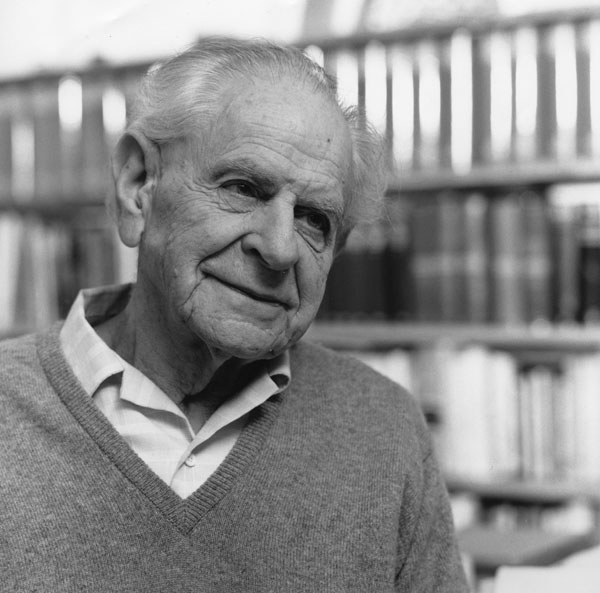
\includegraphics[width=0.65\textwidth]{fig/karl-popper.jpg}
    \caption[Karl Popper]{Porträt von Karl Popper~\cite{PopperPortrait}}
    \label{fig:KarlPopper}
\end{figure}

Karl Popper (siehe auch Abb.~\ref{fig:KarlPopper} auf Seite~\pageref{fig:KarlPopper}) schreibt:

\begin{quote}
"`Wer's nicht einfach und klar sagen kann, der soll schweigen und weiterarbeiten bis er's klar sagen kann."'
\end{quote}

\blindtext

Ein Szenario\footnote{Das ist eine Fußnote.}?

\blindtext

Unter Einbeziehung der Literatur in Kapitel~\ref{chp:LitKrit}, sowie des Gesprächs von Eric Weinstein\footnote{Und eine zweite Fußnote} und Peter Thiel~\cite{WeinsteinThielPortal} \ldots

\blindtext

\blinddescription

\blindtext

\blinditemize

Im Rahmen der Litaraturkritik wurde das Buch (die Bücher) von Byung-Chul Han, \textit{Vom Verschwinden der Rituale}~\cite{HanRituale} gelesen \ldots

Der Podcast zur Vorlesung\footnote{\url{http://podcast.zukunft-denken.eu}} \textit{Zukunft Denken} steht als ergänzende Ressource zur Verfügung.

\blindtext

Scheffer et al beschreiben in ihrem Artikel \ldots ~\cite{SchefferRegimeNature}

\blindtext


%*************************************************************************
%*************************************************************************
\chapter{\LaTeX{} und typographische Anmerkungen} \label{chap:latexRes}

\section{Häufige Fehler} \label{sec:fehler}

\begin{itemize}
    \item \textbf{Spellchecker} nutzen: es wirkt sehr unprofessionell wenn sich Tippfehler etc. im Dokument finden.
    \item Strukturieren des Fließtextes in \textbf{Absätzen}. \textit{Harte Zeilenumbrüche} also \verb+\\+ gibt es im Fließtext niemals. Neuer Absatz in \LaTeX{} wird durch eine Leerzeile zwischen Absätzen ausgelöst.
    \item Absätze werden typographisch auf eine von zwei Möglichkeiten getrennt: mit \textit{Einrückung der ersten Zeile} oder durch \textit{Abstand zwischen den Absätzen}. In der Regel wird ersteres bevorzugt, weil es auch bei Seitenumbrüchen ohne Probleme funktioniert. In \LaTeX{} lässt man schlicht eine Leere Zeile zwischen zwei Absätzen im Quelltext. Das Satzsystem kümmert sich dann um die Typographie des Absatzes. (Keinesfalls aber \verb+\noindent+ oder ähnliches machen.)
    \item Nicht selbst am \textbf{Layout} rumspielen, wenn man sich nicht intensiv mit Typographie beschäftigt hat; z.B. niemals Überschriften mit "`fettem Text"' (also \verb+\textbf{Überschrift}+) machen, sondern die Strukturierung des Dokumentes verwenden.
    \item \textbf{Dokument-Strukturierung} mit: \verb+\part+, \verb+\chapter+, \verb+\section+, \verb+\sub(sub)section+. Die unterste Ebene kann ohne Nummerierung erfolgen: \verb+\paragraph+.
    \item Es gibt \textit{deutsche}, \textit{englische} und \textit{französische} \textbf{Anführungszeichen}. In englischen Texten werden ausschließlich ``englische A'' (\verb+``Text''+) verwendet, im Deutschen "`deutsche"' (\verb+"`Text"'+) oder ">französische As"< (\verb+">Text"<+), niemals englische.
    \item \textbf{Striche} gibt es in drei Arten: Binde-Strich(\verb+-+), 3--4 (\verb+--+) und Gedankenstrich (entweder \verb+---+ bei englischer Typographie oder \verb+ -- + bei deutscher Typographie).
    \item \textbf{Bullet-Punkte} (\verb+\begin{itemize}...\begin{itemize}+ Umgebung) werden für knappe Listen und Aufzählungen verwendet, nicht um Absätze zu strukturieren, dafür verwendet man (sub)sections oder \verb+\paragraph+.
    \item Vorsicht mit \textbf{Satzspiegel-Einstellungen}: (1) richtiges Papierformat wählen (2) Vorsicht mit DIV-Settings. Dieses Template ist vernünftig eingestellt -- im Zweifel diese Einstellungen beibehalten.
    \item \textbf{Zahlen} von 1--12 werden im Deutschen in der Regel ausgeschrieben, also \textit{elf} nicht \textit{11}.
\end{itemize}


\section{Weitere Ressourcen} \label{sec:ressourcen}

\begin{itemize}
    \item \url{https://www.latex-project.org}
    \item \url{https://en.wikibooks.org/wiki/LaTeX}
    \item \url{https://www.overleaf.com}
\end{itemize}




%*************************************************************************
%*************************************************************************
\bibliography{seminararbeit}
\bibliographystyle{plain}

\end{document}
